%===================================================================================
% Chapter: Propuesta para la Extracción de Relaciones
%===================================================================================
\chapter{Propuesta para la Extracción de Relaciones}\label{chapter:relations}
\addcontentsline{toc}{chapter}{Extracción de Relaciones}


\section{Parsing de Dependencias}\label{sec:parsing}

El conocimiento de la estructura y la sint\'axis que subyace en un texto en lenguaje natural puede ser de mucha ayuda en tareas t\'ipicas de NLP como la clasificaci\'on de textos o la sumarizaci\'on. Una de las t\'ecnicas m\'as comunes para capturar cierta estructura en las oraciones es el \emph{parsing}. En esta secci\'on se abordar\'a este tema, particularmente el \emph{parsing} de dependencias.

Hay dos formas de describir la estructura de una oraci\'on en lenguaje natural: separando la oraci\'on en \textbf{constituyentes}~(frases), que se separan a su vez en constituyentes m\'as peque\~nos; o estableciendo conexiones entre las palabras individuales~\cite{covington2001fundamental}. El significado de estas dos variantes se ilustra en las figuras \ref{fig:dep_const} y \ref{fig:dep_links} respectivamente.

\begin{figure}[h!]
	\centering
	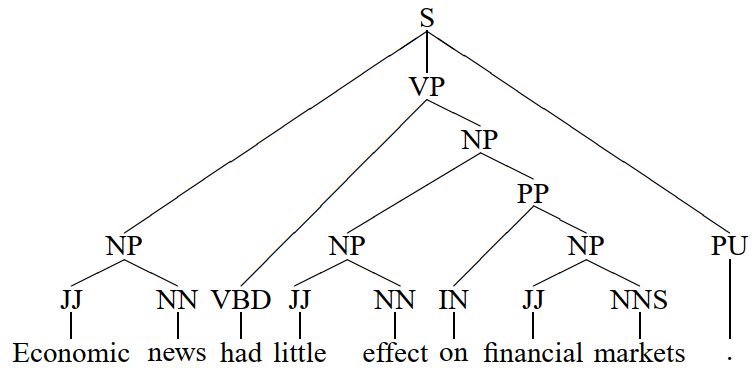
\includegraphics[width=0.8\linewidth]{Graphics/dep_const.png}
	\caption{Estructura constituyente para una oraci\'on en idioma ingl\'es del \emph{Penn Treebank}.}\label{fig:dep_const}
\end{figure}

\begin{figure}[h!]
	\centering
	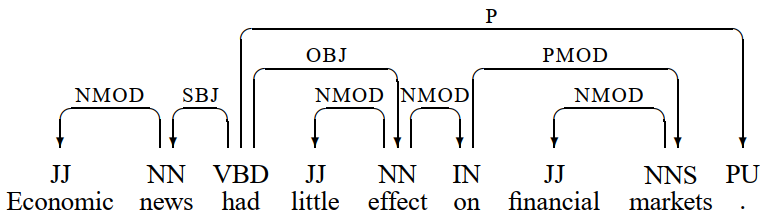
\includegraphics[width=0.8\linewidth]{Graphics/dep_links.png}
	\caption{Estructura de dependencias para una oraci\'on en idioma ingl\'es del \emph{Penn Treebank}.}\label{fig:dep_links}
\end{figure}

La idea de representar de manera constituyente el lenguaje natural tiene muchos a\~nos y ha sido explotada tanto por los cient\'ificos de la computaci\'on como por ling\"uistas, en aras de obtener buenas representaciones del lenguaje natural. Sin embargo, la comunidad cient\'ifica ha mostrado un creciente inter\'es en los \'ultimos a\~nos en las estructuras de dependencias como estrategia para representar las oraciones en lenguaje natural.

La noci\'on fundamental de \textbf{dependencia} est\'a basada en la idea de que la estructura sint\'actica de una oraci\'on est\'a conformada por un conjunto de relaciones binarias asim\'etricas entre las palabras de dicha oraci\'on~\cite{nivre2005dependency}. Siempre que se establece una relaci\'on entre dos palabras, a una de ellas se le denomina \textbf{cabeza} y a la otra \textbf{dependiente}. A continuaci\'on se listan algunos criterios que han sido propuestos para identificar una relaci\'on sint\'actica entre una cabeza $H$ y un dependiente $D$, en una construcci\'on sint\'actica $C~\cite{zwicky1985heads}~\cite{richard1990english}$:

\begin{enumerate}
	\item $H$ determina la categor\'ia sint\'actica de $C$, y muchas veces puede sustituir a $C$.
	
	\item $H$ determina la categor\'ia sem\'antica de $C$, mientras que $D$ aporta especificidad.
	
	\item $H$ es obligatoria, mientra que $D$ es opcional.
	
	\item $H$ selectiona a $D$, y determina si puede o no ser opcional.
	
	\item La forma de $D$ depende de $H$.
	
	\item La posici\'on de $D$ en la oraci\'on se especifica con respecto a $H$.
\end{enumerate}

Estas reglas no son absolutas y contienen un mezcla de criterios variados, algunos sint\'acticos, otros sem\'anticos. No existe en la literatura una noci\'on coherente de dependencia que se corresponda con todos los diferentes criterios~\cite{nivre2005dependency}.


\subsection{Grafo de dependencias}

Si se considera cada dependencia como un arco dirigido que tiene como origen a la cabeza y como destino al dependiente, la estructura de dependecias de la oraci\'on conforma un grafo dirigido $G$ cuyos nodos son los elementos l\'exicos del lenguaje~(\emph{tokens}). Adem\'as, el grafo subyacente de $G$ debe estar conectado, para que cada nodo est\'e relacionado con, al menos, otro nodo.

A esta caracterizaci\'on se le imponen usualmente m\'as restricciones. Dos de las m\'as utilizadas en las distintas formalizaciones de gram\'aticas basadas en dependencias~(o simplemente, gram\'aticas de dependencias), son: la suposici\'on de que cada nodo del grafo tiene \emph{indegree} $\leq 1$; y la no existencia de ciclos en este grafo. Estas suposiciones, junto a la consideraci\'on de conectividad, implican que este grafo sea un \'arbol dirigido con una sola ra\'iz la cual no depende de ninguna otra palabra. Esto \'ultimo queda ilustrado en la figura \ref{fig:dep_tree}. A esta estructura se le denomina \textbf{\'arbol de dependencias}.

\begin{figure}[h!]
	\centering
	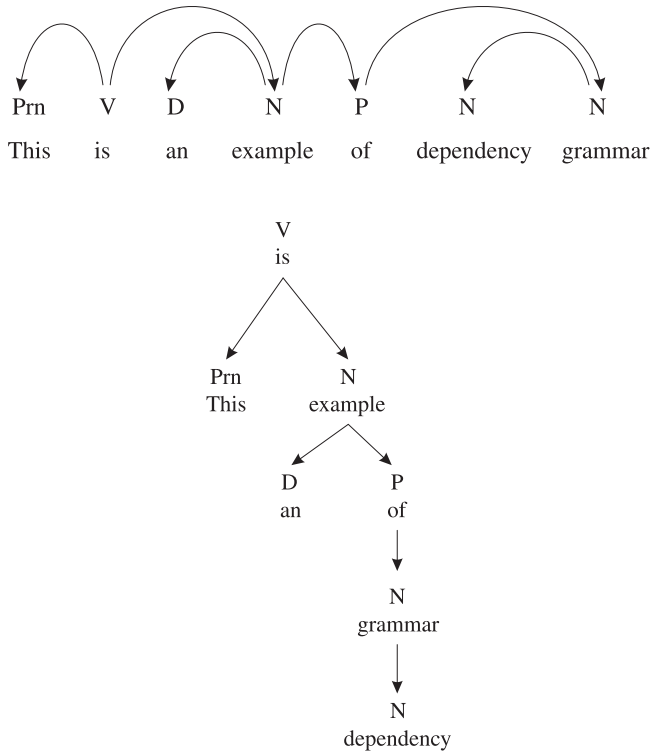
\includegraphics[width=0.7\linewidth]{Graphics/dep_tree.png}
	\caption{Estructura de dependencias para una oraci\'on en idioma ingl\'es y \'arbol de dependencias.}\label{fig:dep_tree}
\end{figure}

Existen varias restricciones adicionales que se definen sobre estas estructuras y que son m\'as debatidas. Una de las m\'as conocidas es la restricci\'on de \textbf{proyectividad}~\cite{hays1964dependency,lecerf1960programme,marcus1965notion}. Un grafo de dependencias satisface la restricci\'on de proyectividad con respecto a un orden linear particular de los nodos si, por cada arco $h \rightarrow d$ y un nodo $w$, $w$ ocurre entre $h$ y $d$ en el orden lineal solo si $w$ est\'a \textbf{dominado} por $h$~\footnote{La relaci\'on \textbf{dominar} es la clausura reflexiva y transitiva de la relaci\'on de dependencia definida por los arcos}. Existen muchos otros aspectos sobre los que se debate que, en aras de mantener la simplicidad, no ser\'an abordados en este trabajo. 

\subsection{Algoritmos para el parsing de dependencias}

Con basamento en estructuras de dependencias, dis\'imiles algoritmos han sido propuestos para \emph{parsear} el lenguaje natural.
De manera general pueden distinguirse dos enfoques diferentes que se han adoptado en la literatura: \emph{parsing} orientado a gram\'aticas y \emph{parsing} orientado a datos. 

Los trabajos pioneros en el \emph{parsing} orientado a gram\'aticas se remontan a las propuestas de Hays y Gaifman, cuando en 1964 y 1965 respectivamente~\cite{hays1964dependency,gaifman1965dependency}, definieron un conjunto de reglas sobre las gram\'aticas de dependencias y un conjunto de condiciones que deb\'ian cumplir las relaciones de dependencia. Por su parte, los primeros intentos en realizar \emph{parsing} de dependencias orientado a datos por Carroll y Charniak (1992)~\cite{carroll1992two}, pueden considerarse tambi\'en orientados a gram\'aticas en el sentido de que apoyaron en el formalismo de una gram\'atica de dependencias y usaron un \emph{corpus} de datos para inducir un modelo probabil\'istico para la desambiguaci\'on. En esencia, usaron una Gram\'atica Libre del Contexto Probabil\'istica~\cite{chomsky1956three}, que estaba restringida para ser equivalente al tipo de gram\'aticas de Hays y Gaifman. 

Muchos otros trabajos se registran en la literatura relativos a propuestas de algoritmos para \emph{parsing} de dependencias~\cite{koo2008simple,mcdonald2005non,nivre2003efficient,nivre2007maltparser,socher2011parsing}. La propuesta m\'as com\'un se basa en alg\'un tipo de algoritmo de programaci\'on din\'amica con o sin desambiguaci\'on estad\'istica.


\subsection{Hipótesis del Camino en el Árbol de Dependencias}


\section{Modelo}\label{sec:model}

La solución propuesta se divide en dos fases.
En un primer momento, para cada par de \textit{tokens} $\langle h1, h2\rangle$ que son cabecera~\footnote{Se le denomina cabecera de una entidad al \textit{token} de menor profundidad de dicha entidad en el árbol de dependencias} de alguna entidad se determina si existe o no una relación desde las entidades cuya cabecera es $h1$  hacia las entidades cuya cabecera es $h2$.
A esta etapa se le denomida reconocimiento.
Seguidamente, para todas las relaciones identificadas se procede a determinar el tipo de dicha relación, proceso denominado clasificación.
Ambos problemas son resueltos a través de modelos de aprendizaje profundo basado en Redes Neuronales Recurrentes sobre estructuras derivadas del árbol de dependencias de la oración en cuestión.

\subsection{Red Neuronal}

La arquitectura definida para la resolución de ambos problemas es similar. 
La entrada de la misma se construye a partir de la secuencia de tokens de la oración, así como de los \textit{tokens} señalados.
La representación de cada token se obtiene a partir de la concatenación de \textit{embeddings} de distintas fuentes de información:

\begin{description}
	\item[Palabras:] Se utilizan \textit{embeddings} preentrenados en un corpus construido a partir de artículos de Wikipedia con contenido médico.
	Fueron entrenados utilizado el algoritmo \textbf{word2vec}\cite{word2vec} con la arquitectura \textbf{skipgram}.
	
	\item[Caracteres:] Se utilizan \textit{embeddings} obtenidos mediante una capa BiLSTM sobre los caracteres de la palabra.
	
	\item[POST-tag y Dependencia:] Se utiliza la un \textit{embedding} de la etiqueta de POS-tag de la palabra y la dependencia de la misma con su ancestro en el árbol de dependencias de la oración.
	
	\item[Etiqueta BMEWO-V y Tipo de la entidad:] Se añaden \textit{embeddings} con información relativa a la entidad a la que pertenece la palabra en cuestión.
	En este caso la etiqueta correspondiente en el sistema BMEWO-V así como el tipo de la entidad.
	
\end{description}

El procesamiento de la entrada lo realizan dos componentes: una capa BiLSTM y otra LSTM apiladas, y una capa Tree-LSTM; que operan sobre estructuras derivadas del árbol de dependencias de la oración.

\begin{description}
	\item[LSTM:] Las LSTM son un tipo de Red Neuronal Recurrente (RNN), donde en la capa oculta, las actualizaciones son reemplazadas por células de memoria especialmente diseñadas.
	Como resultado pueden ser mejores encontrando y explotando amplios rangos de dependencia en los datos~\cite{hochreiter1997long}.
	
	\item[BiLSTM:] En tareas en las que resulta conveniente tener acceso a rasgos pasados y futuros (como son las palabras que hay antes y después de otra palabra en una oración) se puede utilizar una red LSTM bidireccional, conocida como BiLSTM~\cite{graves2013speech}.
	Tradicionalmente las redes BiLSTM se entrenan usando propagación hacia atrás a través del tiempo~\cite{boden2002guide}.
	
	\item[Tree-LSTM:]
	Las redes Tree-LSTM son una generalización de la arquitectura LSTM. 
	Mientras la red LSTM tradicional computa su estado a partir de la entrada en el momento actual y el estado de la célula LSTM en el momento anterior, las Tree-LSTM lo realizan a partir del vector de entrada y los estados de una cantidad arbitraria de hijos~\cite{tai2015improved}.
	Estas redes han sido utilizadas previamente para representar estructuras sintácticas de de un oración~\cite{miwa2016end}.
	
\end{description}

Las capas recurrentes apiladas obtienen una representación de la secuencia de \textit{tokens} que aparecen en el árbol de dependencias, en el camino entre los \textit{tokens} señalados.
Entre tanto, la capa Tree-LSTM obtiene una representación del subárbol que tiene como raíz a cada \textit{token} señalado, respectivamente.

Estos tres vectores se concatentan y pasan por un clasificador constituído por una capa densa. 
En la etapa de reconocimiento, el clasificador es binario con función de activación \textit{sigmoid}.
Mientras que para la etapa de clasificación, se obtiene una distribución de probabilidades sobre el conjunto de relaciones mediante una función de activación \textit{softmax}.

La figura \ref{fig:rel_model} ilustra la arquitectura descrita para la etapa de clasificación.

\begin{figure}[h!]
	\centering
	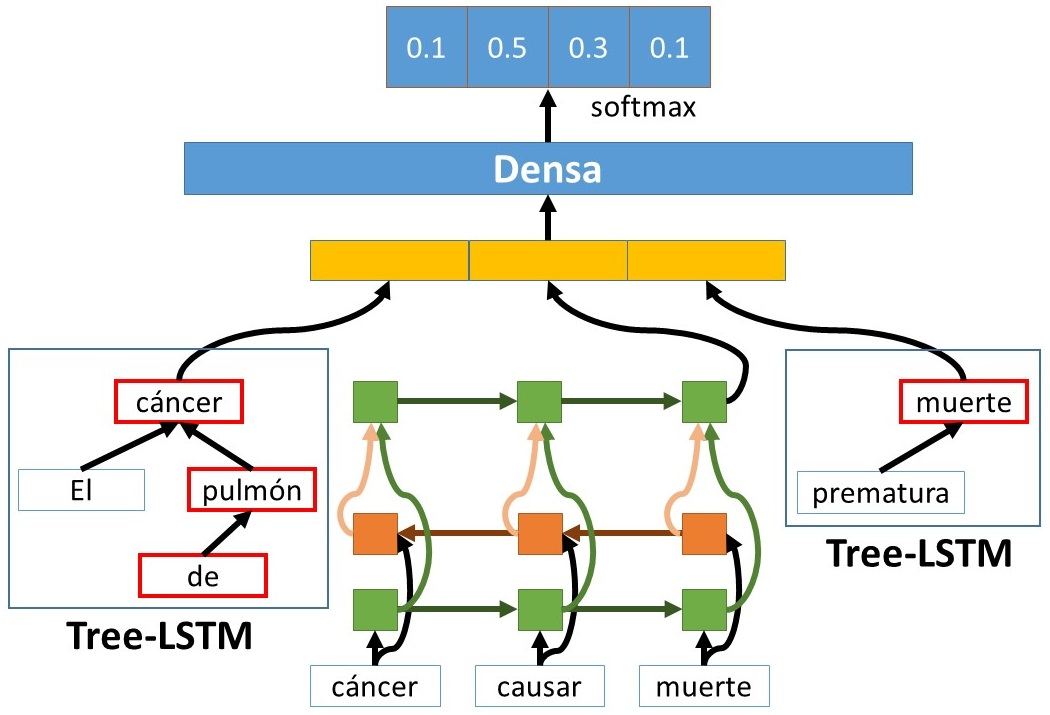
\includegraphics[width=1\linewidth]{Graphics/rel_model_class.jpg}
	\caption{Arquitectura de red utilizada. La oración de entrada es \textit{El cáncer de pulmón puede causar muerte prematura} Y las entidades en cuestión son \textit{cáncer de pulmón} y \textit{muerte}.}\label{fig:rel_model}
\end{figure}

%===================================================================================